\chapter{Saving your work}
\label{ch:saving_your_work}

\newthought{At the end of a lesson}, your workflow may look like this:
\begin{figure}[h]
  \centering
  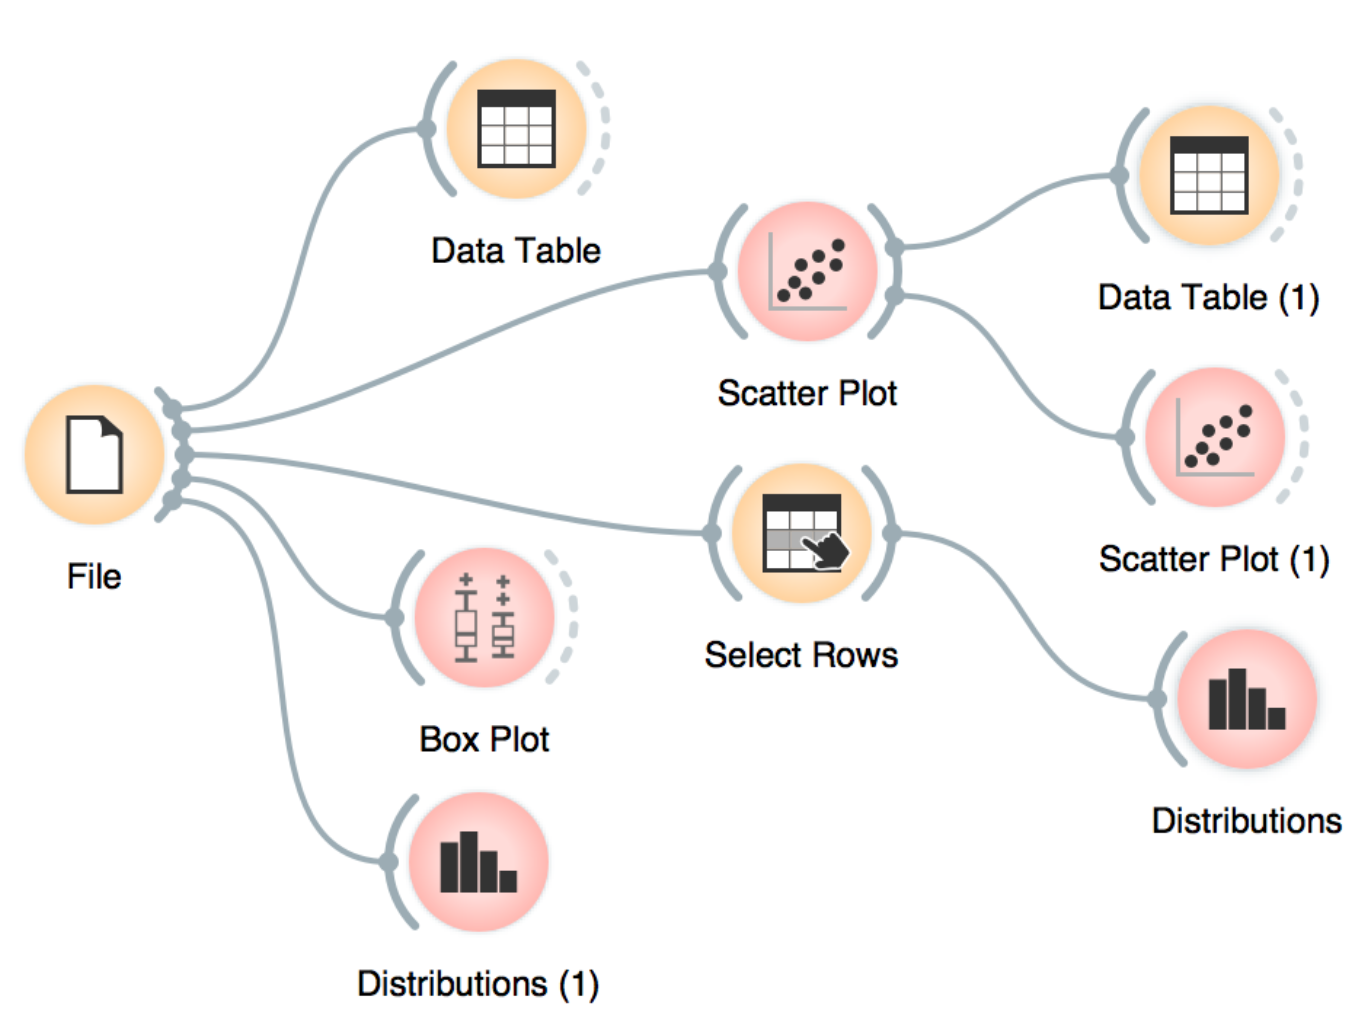
\includegraphics[width=65mm]{saving-fig1.png}%
  \caption{A fairly complex workflow that you would want to share or reuse at a later time.}
  \label{fig:saveing-fig1}
\end{figure}

You can save this workflow, otherwise called a "\textit{Schema}" using the File/Save menu and share it with your colleagues. Just don't forget to put the data files in the same directory as the file with the workflow.

Widgets also have a Report button in their bottom status bar, which you can use to keep a log of your analysis. When you find something interesting, just click it and the graph\marginnote{Clicking on a section of the report window allows you to add a comment.} will be added to your log. You can also add reports from the widgets on the path to this one, to make sure you don't forget anything relevant.

\begin{marginfigure}
  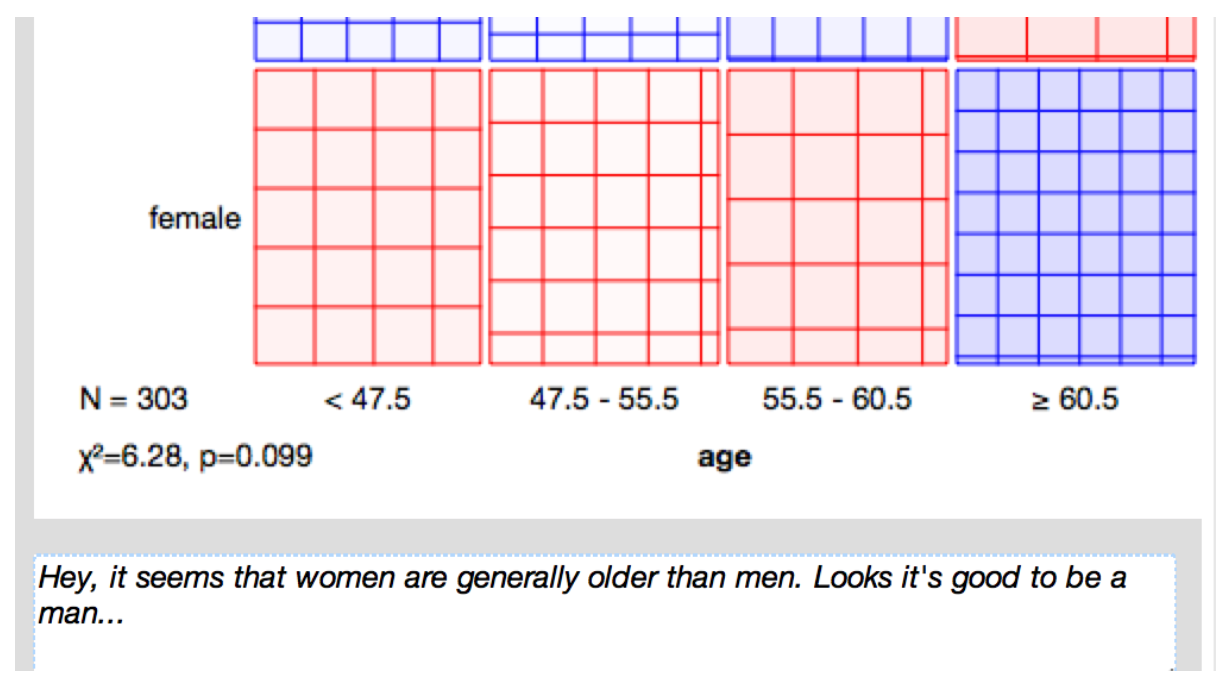
\includegraphics[width=60mm]{saving-fig3.png}%
  \caption{The report window (left) and the additional text input box (top).}
  \label{fig:saveing-fig3}
\end{marginfigure}

\begin{figure}[h]
  \centering
  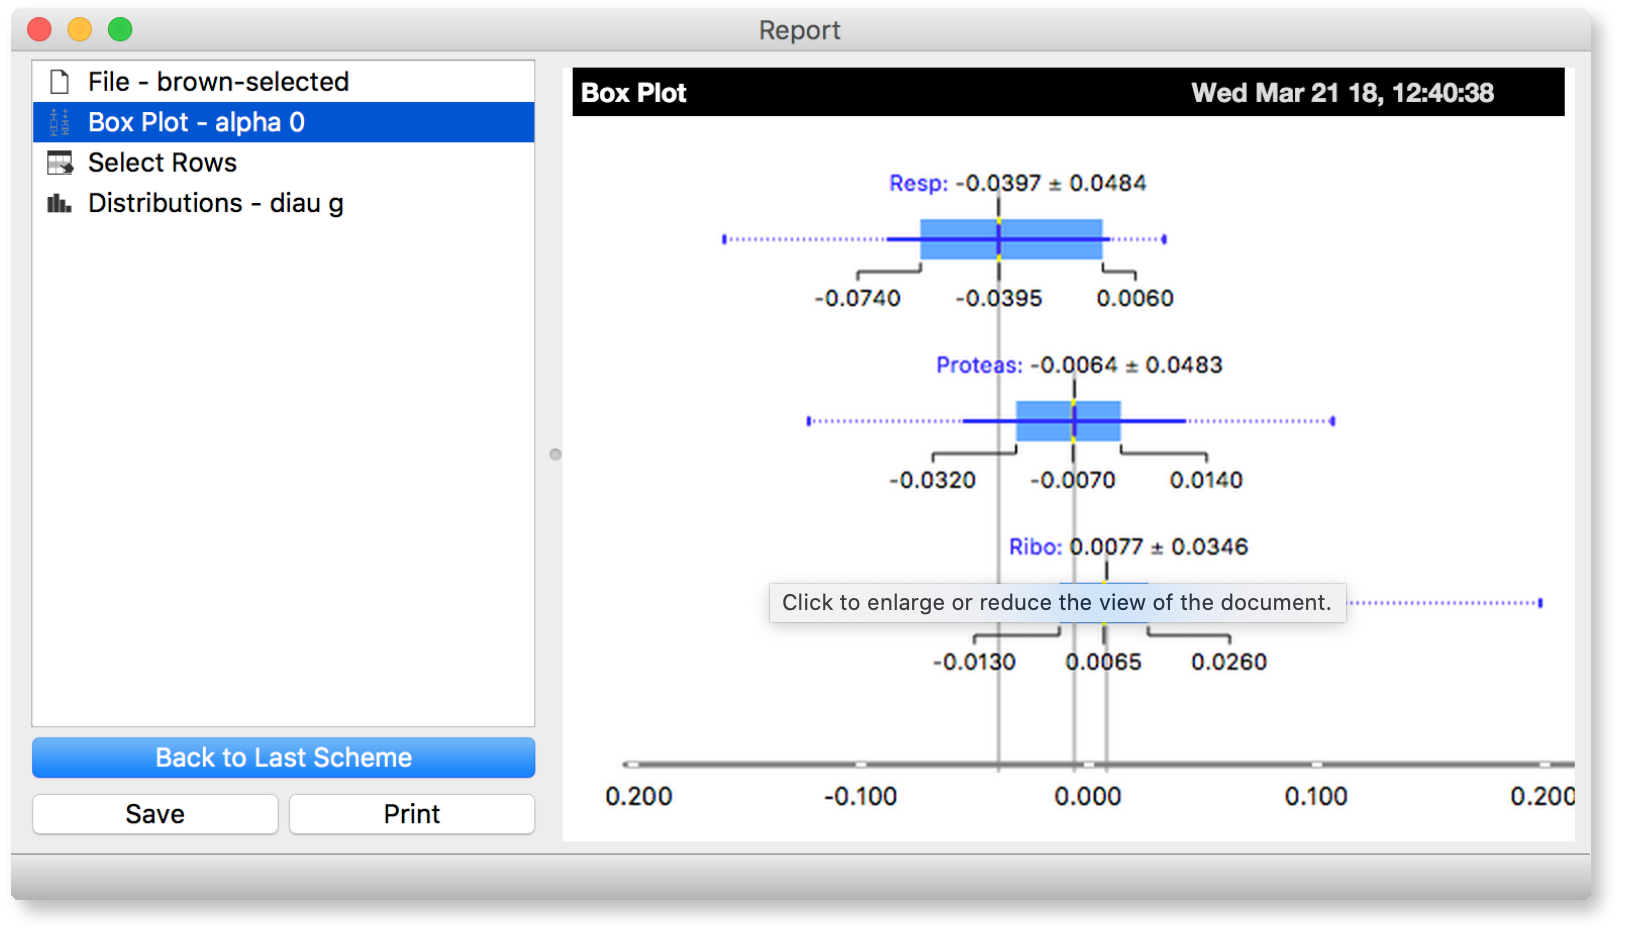
\includegraphics[width=\linewidth]{saving-fig2.png}%
  \label{fig:saveing-fig2}
\end{figure}

You can save the report as HTML or PDF, or a report file that includes all workflow related report items that you can later open in Orange. In this way, you and your colleagues can reproduce your analysis results.